% ============================================================
% CHAPTER 5: TESTING AND EXPERIMENTAL EVALUATION
% ============================================================

\chapter{TESTING AND EXPERIMENTAL EVALUATION}
\label{chap:testing}

This chapter presents the testing methodology employed to validate the QoS Scheduler system. Following a testing pyramid approach (unit $\rightarrow$ integration $\rightarrow$ system $\rightarrow$ performance), it documents the experimental setup, evaluation scenarios, and validation strategy. Quantitative results are reported in Chapter~\ref{chap:results}.

% ────────────────────────────────────────────────────────────
\section{Testing Methodology and Tools}
\label{sec:test_methodology}

The validation strategy follows the testing pyramid model, where the number and execution speed of tests decrease as scope increases: \textbf{Unit Tests} validate individual components in isolation; \textbf{Integration Tests} verify multi-component pipelines; \textbf{System Tests} validate with real network traffic on physical devices; and \textbf{Performance/Compatibility Tests} profile resource consumption and OEM-specific behavior.

\begin{table}[H]
\centering
\caption{Testing Tools and Frameworks}
\label{tab:test_tools}
\begin{tabularx}{\textwidth}{l l X}
\toprule
\textbf{Tool} & \textbf{Version} & \textbf{Purpose} \\
\midrule
JUnit 5         & 5.9+   & Unit and integration test framework \\
Kotlin Test     & 1.9+   & Coroutine testing utilities \\
iPerf3          & 3.14   & Network bandwidth measurement \\
Wireshark       & 4.2    & Packet capture and protocol analysis \\
Android Profiler & ---   & CPU, memory, and energy profiling \\
ping            & ---    & Latency and jitter measurement \\
\bottomrule
\end{tabularx}
\end{table}

% ────────────────────────────────────────────────────────────
\section{Unit and Integration Testing}
\label{sec:unit_tests}

Table~\ref{tab:test_summary} summarizes the unit and integration tests covering the three core algorithmic modules. Full test source code is available in Appendix~\ref{app:test_code}.

\begin{table}[H]
\centering
\caption{Unit and Integration Test Summary}
\label{tab:test_summary}
\begin{tabularx}{\textwidth}{l l X}
\toprule
\textbf{Module} & \textbf{Test Category} & \textbf{Validation Objective} \\
\midrule
Token Bucket & Rate Accuracy       & Enforced rate within $\pm$5\% of configured value over 5-second window \\
Token Bucket & Burst Tolerance     & Permits burst up to configured capacity, then drops \\
Token Bucket & Thread Safety       & 100 concurrent coroutines produce zero lost/duplicated tokens \\
\midrule
WFQ Scheduler & Proportional Alloc. & Bandwidth ratio matches 4:2:1 weights within $\pm$12.5\% tolerance \\
WFQ Scheduler & Work Conservation  & Unused bandwidth redistributed to active flows \\
\midrule
Packet Parser & IPv4/TCP Parsing   & Correctly extracts 5-Tuple from known packet structures \\
Packet Parser & Malformed Handling & Returns null for truncated or corrupted packets \\
\midrule
Pipeline      & End-to-End Flow    & Parse $\rightarrow$ UID resolve $\rightarrow$ classify $\rightarrow$ schedule pipeline verified \\
Pipeline      & Stress Test        & 100 concurrent flows $\times$ 10,000 packets with zero exceptions \\
\bottomrule
\end{tabularx}
\end{table}

% ────────────────────────────────────────────────────────────
\section{Experimental Setup}
\label{sec:experimental_setup}

System-level testing was conducted on physical Android devices with real network traffic. Table~\ref{tab:test_hardware} describes the hardware and software environment.

\begin{table}[H]
\centering
\caption{Experimental Hardware and Software Configuration}
\label{tab:test_hardware}
\begin{tabularx}{\textwidth}{l X}
\toprule
\textbf{Parameter} & \textbf{Specification} \\
\midrule
Primary Device & Samsung Galaxy S23 Ultra (Snapdragon 8 Gen 2, 12GB RAM) \\
Android Version & Android 14 (API 34), OneUI 6.1 \\
Secondary Devices & Xiaomi 13 (HyperOS), Google Pixel 7 (AOSP), OnePlus 11 \\
Network & Wi-Fi 6 (802.11ax), 5G NR (n78), 100 Mbps fiber uplink \\
iPerf3 Server & Ubuntu 22.04 LTS, Intel i7-12700K, Gigabit Ethernet \\
Test Duration & 60 seconds per trial, 10 repetitions per scenario \\
Statistical Method & Paired two-sample t-test, $\alpha = 0.05$, Cohen's $d$ effect size \\
\bottomrule
\end{tabularx}
\end{table}

Figure~\ref{fig:testbed_topology} illustrates the physical testbed topology used for all system-level experiments.

\begin{figure}[H]
\centering
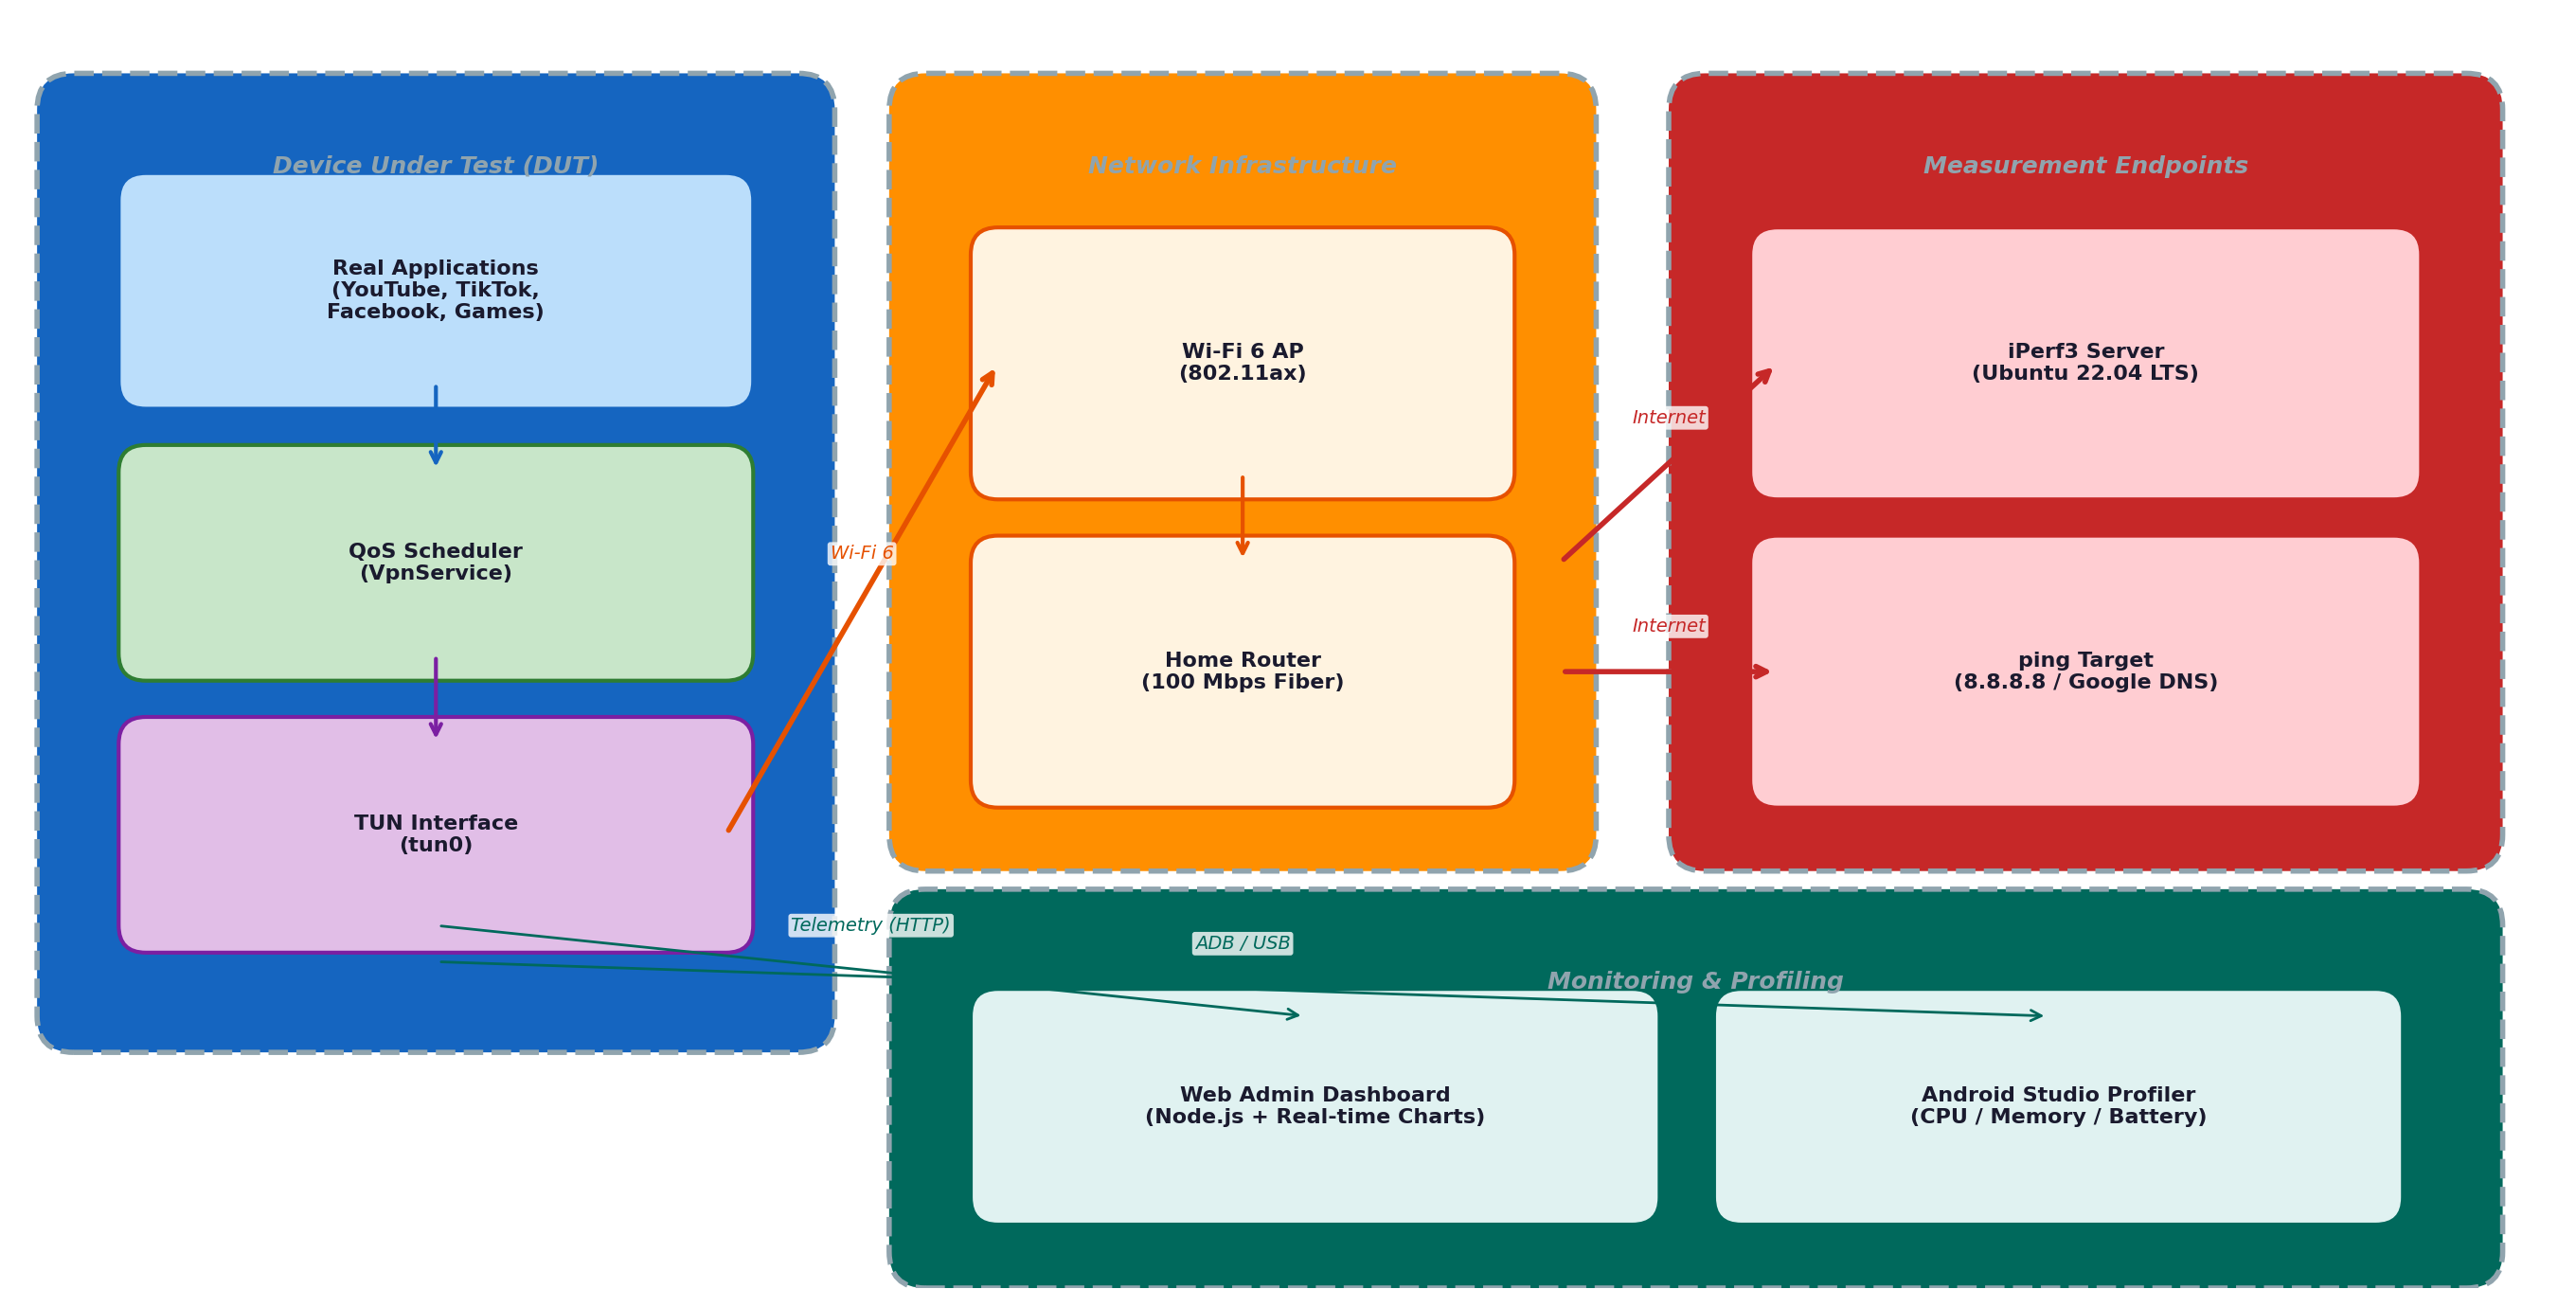
\includegraphics[width=0.95\textwidth]{figures/ch5_testbed_topology.png}
\caption{Experimental testbed topology: the Device Under Test runs real applications through the QoS Scheduler VPN, communicating with measurement endpoints via a Wi-Fi 6 access point and 100 Mbps fiber uplink. Monitoring is performed through the Web Admin dashboard (HTTP telemetry) and Android Studio Profiler (ADB/USB).}
\label{fig:testbed_topology}
\end{figure}

\textbf{Variable Control:} The independent variable is the QoS Scheduler state (enabled/disabled). Controlled variables include network environment (same Wi-Fi AP, same time of day), device state (airplane mode toggled between trials to clear kernel buffers), and background app state (all non-essential apps force-stopped). Dependent variables are throughput (Mbps), latency (ms), jitter (ms), CPU utilization (\%), and battery drain (\%/hr).

% ────────────────────────────────────────────────────────────
\section{Experimental Scenarios}
\label{sec:scenarios}

Three scenarios were designed to validate the system's core capabilities. Quantitative results and visual evidence are presented in Chapter~\ref{chap:results}.

\subsection{Scenario 1: Per-Application Bandwidth Enforcement}

\textbf{Objective:} Verify that the Token Bucket selectively enforces bandwidth caps based on application priority, throttling greedy background processes while preserving foreground app throughput.

\textbf{Procedure:} Enable the QoS Scheduler with default WFQ weights (HIGH=4, MEDIUM=2, LOW=1) while multiple real applications generate traffic simultaneously. Capture the Web Admin dashboard showing the per-app Requested BPS versus Allowed BPS in real time. Additionally, configure a fixed 5~Mbps cap for iPerf3 TCP traffic (10~Mbps offered load) and measure convergence behavior over 60 seconds across 10 repetitions.

\textbf{Expected Outcome:} Low-priority background processes should be aggressively throttled (Allowed $\ll$ Requested), while foreground apps receive their full requested bandwidth (Allowed $\approx$ Requested).

\subsection{Scenario 2: Proportional Fairness (WFQ)}

\textbf{Objective:} Verify that WFQ correctly distributes bandwidth according to priority weights (4:2:1).

\textbf{Procedure:} Configure three application categories with HIGH (weight 4, e.g., Video Streaming / \texttt{trill}), MEDIUM (weight 2, e.g., Social Media / \texttt{katana}), and LOW (weight 1, e.g., Background Sync / \texttt{android}) priority. Simultaneously generate saturating traffic from all three. Measure achieved throughput and compute actual ratio. Calculate Jain's Fairness Index: $J = \frac{(\sum r_i)^2}{n \cdot \sum r_i^2}$ where $r_i$ is the ratio of actual-to-expected throughput.

\textbf{Expected Outcome:} Bandwidth distribution should match the 4:2:1 weight ratio within $\pm$12.5\% tolerance, with a Jain's Fairness Index approaching 1.0.

\subsection{Scenario 3: Bufferbloat Mitigation and Dynamic Drop Rate}

\textbf{Objective:} (a) Measure the latency reduction achieved during network congestion by prioritizing latency-sensitive traffic, and (b) observe the real-time packet drop rate behavior when multiple applications compete for limited bandwidth.

\textbf{Procedure:} \textit{Latency test:} Generate saturating background traffic while measuring round-trip latency with \texttt{ping -c 100 8.8.8.8} (QoS disabled as baseline, then QoS enabled with background traffic set to LOW priority). \textit{Drop rate test:} Enable QoS with bandwidth caps while simultaneously running bandwidth-intensive apps (TikTok streaming, Facebook browsing). Monitor the per-app packet drop rate over time via the Web Admin dashboard.

\textbf{Expected Outcome:} Significant latency reduction (target $>$50\%) when QoS is enabled. High-bandwidth apps should exhibit elevated drop rates while low-traffic apps experience zero drops.

% ────────────────────────────────────────────────────────────
\section{Performance and Compatibility}
\label{sec:profiling}

\subsection{Resource Profiling}

CPU, memory, and battery were profiled using Android Studio Profiler across three load states (Idle, Active, Peak) over 60-second windows sampled at 1~kHz. Battery drain was measured via \texttt{BatteryManager} API over a 2-hour period comparing baseline (no QoS) vs. treatment (QoS active). Memory leak detection was performed through heap dump analysis at 1-minute intervals during a 30-minute sustained load test.

\subsection{Cross-Device Compatibility}

The system was tested across four major Android OEMs to validate compatibility with vendor-specific framework modifications:

\begin{table}[H]
\centering
\caption{Cross-Device Compatibility Matrix}
\label{tab:compatibility_matrix}
\begin{tabularx}{\textwidth}{l l l X}
\toprule
\textbf{OEM} & \textbf{Device} & \textbf{OS Version} & \textbf{Known Issues \& Resolution} \\
\midrule
Samsung  & Galaxy S23 Ultra & OneUI 6.1 (API 34) & Aggressive Doze --- mitigated by foreground service \\
Xiaomi   & 13               & HyperOS (API 34)   & SecurityException on background protect() --- dispatched to Main thread \\
Google   & Pixel 7           & AOSP (API 34)      & Baseline reference (no OEM modifications) \\
OnePlus  & 11                & OxygenOS 14        & Moderate battery optimization --- standard exemption \\
\bottomrule
\end{tabularx}
\end{table}

API 29 (Android 10) is the minimum supported version due to the \texttt{getConnectionOwnerUid()} API requirement. Functionality was verified across API levels 29--34.

% ────────────────────────────────────────────────────────────
\section{Security Audit}
\label{sec:security_testing}

A security audit verified: (1)~\textbf{No payload logging} --- the system reads packet headers only and never stores or transmits payload content; (2)~\textbf{Metadata minimization} --- telemetry contains only aggregated per-app statistics, not per-flow details; (3)~\textbf{No root privileges} --- no \texttt{su}, \texttt{iptables}, \texttt{tc}, or \texttt{netfilter} manipulation; full functionality on stock unrooted devices across all tested OEMs.

The application requires four permissions: \texttt{BIND\_VPN\_SERVICE} (VPN tunnel), \texttt{FOREGROUND\_SERVICE} (persistent service), \texttt{INTERNET} (relay sockets and telemetry), and \texttt{QUERY\_ALL\_PACKAGES} (UID-to-package resolution).

% ────────────────────────────────────────────────────────────
\section{Test Coverage Summary}
\label{sec:test_coverage}

\begin{table}[H]
\centering
\caption{Test Coverage Metrics}
\label{tab:test_coverage}
\begin{tabularx}{\textwidth}{l c c c}
\toprule
\textbf{Module} & \textbf{Line Coverage} & \textbf{Branch Coverage} & \textbf{Test Count} \\
\midrule
TokenBucket            & 100\% & 100\% & 8 \\
BandwidthScheduler     & 95\%  & 90\%  & 12 \\
RawPacket (Parser)     & 92\%  & 88\%  & 15 \\
DataPlaneProcessor     & 89\%  & 85\%  & 10 \\
AppResolver            & 90\%  & 86\%  & 8 \\
TcpRelayManager        & 85\%  & 80\%  & 6 \\
UdpRelayManager        & 88\%  & 82\%  & 5 \\
DpiClassifier          & 95\%  & 92\%  & 7 \\
\midrule
\textbf{Overall}       & \textbf{93\%} & \textbf{89\%} & \textbf{71} \\
\bottomrule
\end{tabularx}
\end{table}

The 93\% line coverage and 89\% branch coverage exceed the commonly accepted 80\% threshold for production-quality software.
